% To produce pdf under linux, run
% pdflatex HW2.tex 
  
\documentclass{article}
\usepackage{amsmath,amssymb}
\usepackage{graphicx}
\usepackage{url}
\usepackage{listings}
\usepackage{color}
\usepackage{upquote}
\usepackage{courier}
\usepackage{caption}
\usepackage{verbatim} 
\usepackage{hyperref}
\usepackage{qtree}
\newcommand\Colorhref[3][blue]{\href{#2}{\small\color{#1}#3}}

\usepackage{array}
\setlength\arrayrulewidth{.4pt}
\setlength\tabcolsep{3pt}
\newcolumntype{L}[1]{>{\centering\let\newline\\\arraybackslash\hspace{0pt}}m{#1}}
\newcolumntype{C}[1]{>{\centering\let\newline\\\arraybackslash\hspace{0pt}}m{#1}}
\newcolumntype{R}[1]{>{\centering\let\newline\\\arraybackslash\hspace{0pt}}m{#1}}
\newcolumntype{M}[1]{>{\centering\let\newline\\\arraybackslash\hspace{0pt}}m{#1}}

\definecolor{dkgreen}{rgb}{0,0.6,0}
\definecolor{gray}{rgb}{0.5,0.5,0.5}
\definecolor{mauve}{rgb}{0.58,0,0.82}

\lstset{frame=shadowbox,
	rulesepcolor=\color{black},
  	language=bash,
  	aboveskip=3mm,
  	belowskip=3mm,
  	showstringspaces=false,
  	columns=flexible,
  	basicstyle={\small\ttfamily},
  	numbers=none,
  	numberstyle=\tiny\color{gray},
  	keywordstyle=\color{blue},
  	commentstyle=\color{dkgreen},
  	stringstyle=\color{red},
  	breaklines=true,
  	breakatwhitespace=true
  	tabsize=3
}
\title{Algorithm Assignment 1}
\author{Seshagiri Prabhu}

\begin{document}
\maketitle
\begin{center}
\href{mailto:seshagiriprabhu@gmail.com}{seshagiriprabhu@gmail.com}
\end{center}
\date{}

\section{Write a program to multiply two matrices of NxN using naïve algorithm}
\begin{lstlisting}
# /usr/bin/python

from gmpy import mpq,mpz
from random import randint,seed
from time import time

def rand_matrix(n, typ=int, N=10):
    ''' A function to matrix with random elements '''

    m = []
    for i in range(n):
        a = []

        for j in range(n):
            p = randint(0, N)
            a.append(p)

        m.append(a)
    return m

def matrixmult (A, B):
    ''' A function to do normal matrix multiplication '''

    rows_A = len(A)
    cols_A = len(A[0])
    rows_B = len(B)
    cols_B = len(B[0])

    if cols_A != rows_B:
      print "Cannot multiply the two matrices. Incorrect dimensions."
      return

    # Create the result matrix
    # Dimensions would be rows_A x cols_B
    C = [[0 for row in range(cols_B)] for col in range(rows_A)]

    for i in range(rows_A):        # C * n
        for j in range(cols_B):    # C * n * n
            for k in range(cols_A):  # C * n * n
                C[i][j] += A[i][k]*B[k][j]
    return C

def test_1(N):
    seed(2)
    for n in range(100, 1000, 100):
        a = rand_matrix(n, mpq, N)
        b = rand_matrix(n, mpq, N)
        t0 = time()
        C = matrixmult(a, b)
        t1 = time()

        print 'dimension: %d traditional way: %.2f' %(n, t1-t0)

test_1(1000000)
\end{lstlisting}

Time complexity: $O(n^{3})$\\

\section{Strassen multiplication Algorithm}
\begin{lstlisting}
# /usr/bin/python

from gmpy import mpq,mpz
from random import randint,seed
from time import time

def rand_matrix(n, typ=int, N=10):
    ''' A function to matrix with random elements '''

    m = []
    for i in range(n):
        a = []

        for j in range(n):
            p = randint(0, N)
            a.append(p)

        m.append(a)
    return m

def madd(a, b):
    ''' A function to add two matrices '''

    n = len(a)
    c = []

    for i in range(n):
        c.append(a[i][:])

    for i in range(n):
        c1 = c[i]
        b1 = b[i]

        for j in range(n):
            c1[j] += b1[j]

    return c


def imadd(a, b):
    ''' A function to '''

    n = len(a)
    for i in range(n):
        a1 = a[i]
        b1 = b[i]

        for j in range(n):
            a1[j] += b1[j]

    return a

def msub(a, b):
    ''' A function to substract two matrices '''

    n = len(a)
    c = []
    for i in range(n):
        c.append(a[i][:])

    for i in range(n):
        c1 = c[i]
        b1 = b[i]
        for j in range(n):
            c1[j] -= b1[j]

    return c

def imsub(a, b):
    ''' A function to substract two matrices'''

    n = len(a)
    for i in range(n):
        a1 = a[i]
        b1 = b[i]
        for j in range(n):
            a1[j] -= b1[j]
    return a

def mmul(a, b):
    ''' A function to multiply two matrices in a traditional way '''

    n = len(a)
    c = []

    for i in range(n):
        cv = []
        a1 = a[i]

        for j in range(n):
            r = 0

            for k in range(n):
                r += a1[k] * b[k][j]

            cv.append(r)
        c.append(cv)
    return c

def mmul(a, b, trans=0):
    ''' A function to multiply transitive matrices '''

    n = len(a)
    c = []
    if not trans:
        bt = [[0]*n for _ in range(n)]

        for i in range(n):
            for j in range(n):
                bt[i][j] = b[j][i]

        b = bt

    for i in range(n):
        a1 = a[i]
        cv = []
        for j in range(n):
            b1 = b[j]
            r = 0
            for k in range(n):
                r += a1[k]*b1[k]
            cv.append(r)
        c.append(cv)
    return c

def strassen_mul(a,b,trans=0):
    ''' Strassem multiply implementation '''

    n = len(a)
    if n % 2 == 1 or n <= 128:
        return mmul(a,b,trans)

    rn0 = range(n/2)
    rn1 = range(n/2, n)
    A00 = [a[i] [:n/2] for i in rn0]
    A01 = [a[i] [n/2:] for i in rn0]
    A10 = [a[i] [:n/2] for i in rn1]
    A11 = [a[i] [n/2:n] for i in rn1]

    if trans:
        B00 = [b[i] [:n/2] for i in rn0]
        B10 = [b[i] [n/2:] for i in rn0]
        B01 = [b[i] [:n/2] for i in rn1]
        B11 = [b[i] [n/2:n] for i in rn1]

    else:
        B00 = [[b[j][i] for j in rn0] for i in rn0]
        B01 = [[b[j][i] for j in rn0] for i in rn1]
        B10 = [[b[j][i] for j in rn1] for i in rn0]
        B11 = [[b[j][i] for j in rn1] for i in rn1]

    M1 = strassen_mul(madd(A00, A11), madd(B00, B11), 1)
    M2 = strassen_mul(madd(A10, A11), B00, 1)
    M3 = strassen_mul(A00, msub(B01, B11), 1)
    M4 = strassen_mul(A11, msub(B10, B00), 1)
    M5 = strassen_mul(madd(A00, A01), B11, 1)
    M6 = strassen_mul(msub(A10, A00), madd(B00, B01), 1)
    M7 = strassen_mul(msub(A01, A11), madd(B10, B11), 1)
    C00 = madd(msub(madd(M1, M4), M5), M7)
    C01 = madd(M3, M5)
    C10 = madd(M2, M4)
    C11 = madd(madd(msub(M1, M2), M3), M6)
    c = [C00[i] + C01[i] for i in rn0]
    for i in rn0:
        c.append(C10[i] + C11[i])
    return c


def test_1(N):
    seed(2)
    for n in range(100, 1000, 100):
        a = rand_matrix(n, mpq, N)
        b = rand_matrix(n, mpq, N)
        t0 = time()
        C = mmul(a, b)
        t1 = time()
        c = strassen_mul(a,b)
        t2 = time()
        assert c == C
        print 'dimension=%d traditional way: %.2f strassen: %.2f' %(n, t1-t0, t2-t1)

test_1(1000000)
\end{lstlisting}


Time complexity: $O(n^{2.807})$

\section{Implementation of the program}
The implementation of my program is available in my \Colorhref{https://github.com/seshagiriprabhu/advanced-computer-algorithm}{github} (under matrix directory) repository.

\section{Graph}
\begin{flushright}
	\begin{tabular}{| L{4cm} | C{4cm} | R{4cm} |}
		\hline \textbf{Input Size} & \textbf{Naive approach} & \textbf{Strassen}   \\
		\hline 100 & 0 & 0 \\
		\hline 100 & 0.21 & 0.21 \\
		\hline 200 & 1.67 & 1.56 \\
		\hline 300 & 5.64 & 4.73 \\
		\hline 400 & 13.94 & 11.36 \\
		\hline 500 & 27.73 & 21.64 \\
		\hline 600 & 47.96 & 34.03 \\
		\hline 700 & 81.39 & 60.78 \\
		\hline 800 & 124.36 & 84.36 \\
		\hline 900 & 177.66 & 127.86 \\
		\hline 1000 & 232.52 & 151.30 \\
		\hline 1100 & 311.57 & 232.37 \\
		\hline
	\end{tabular}	
\end{flushright}

\section{Graph}
\begin{flushleft}
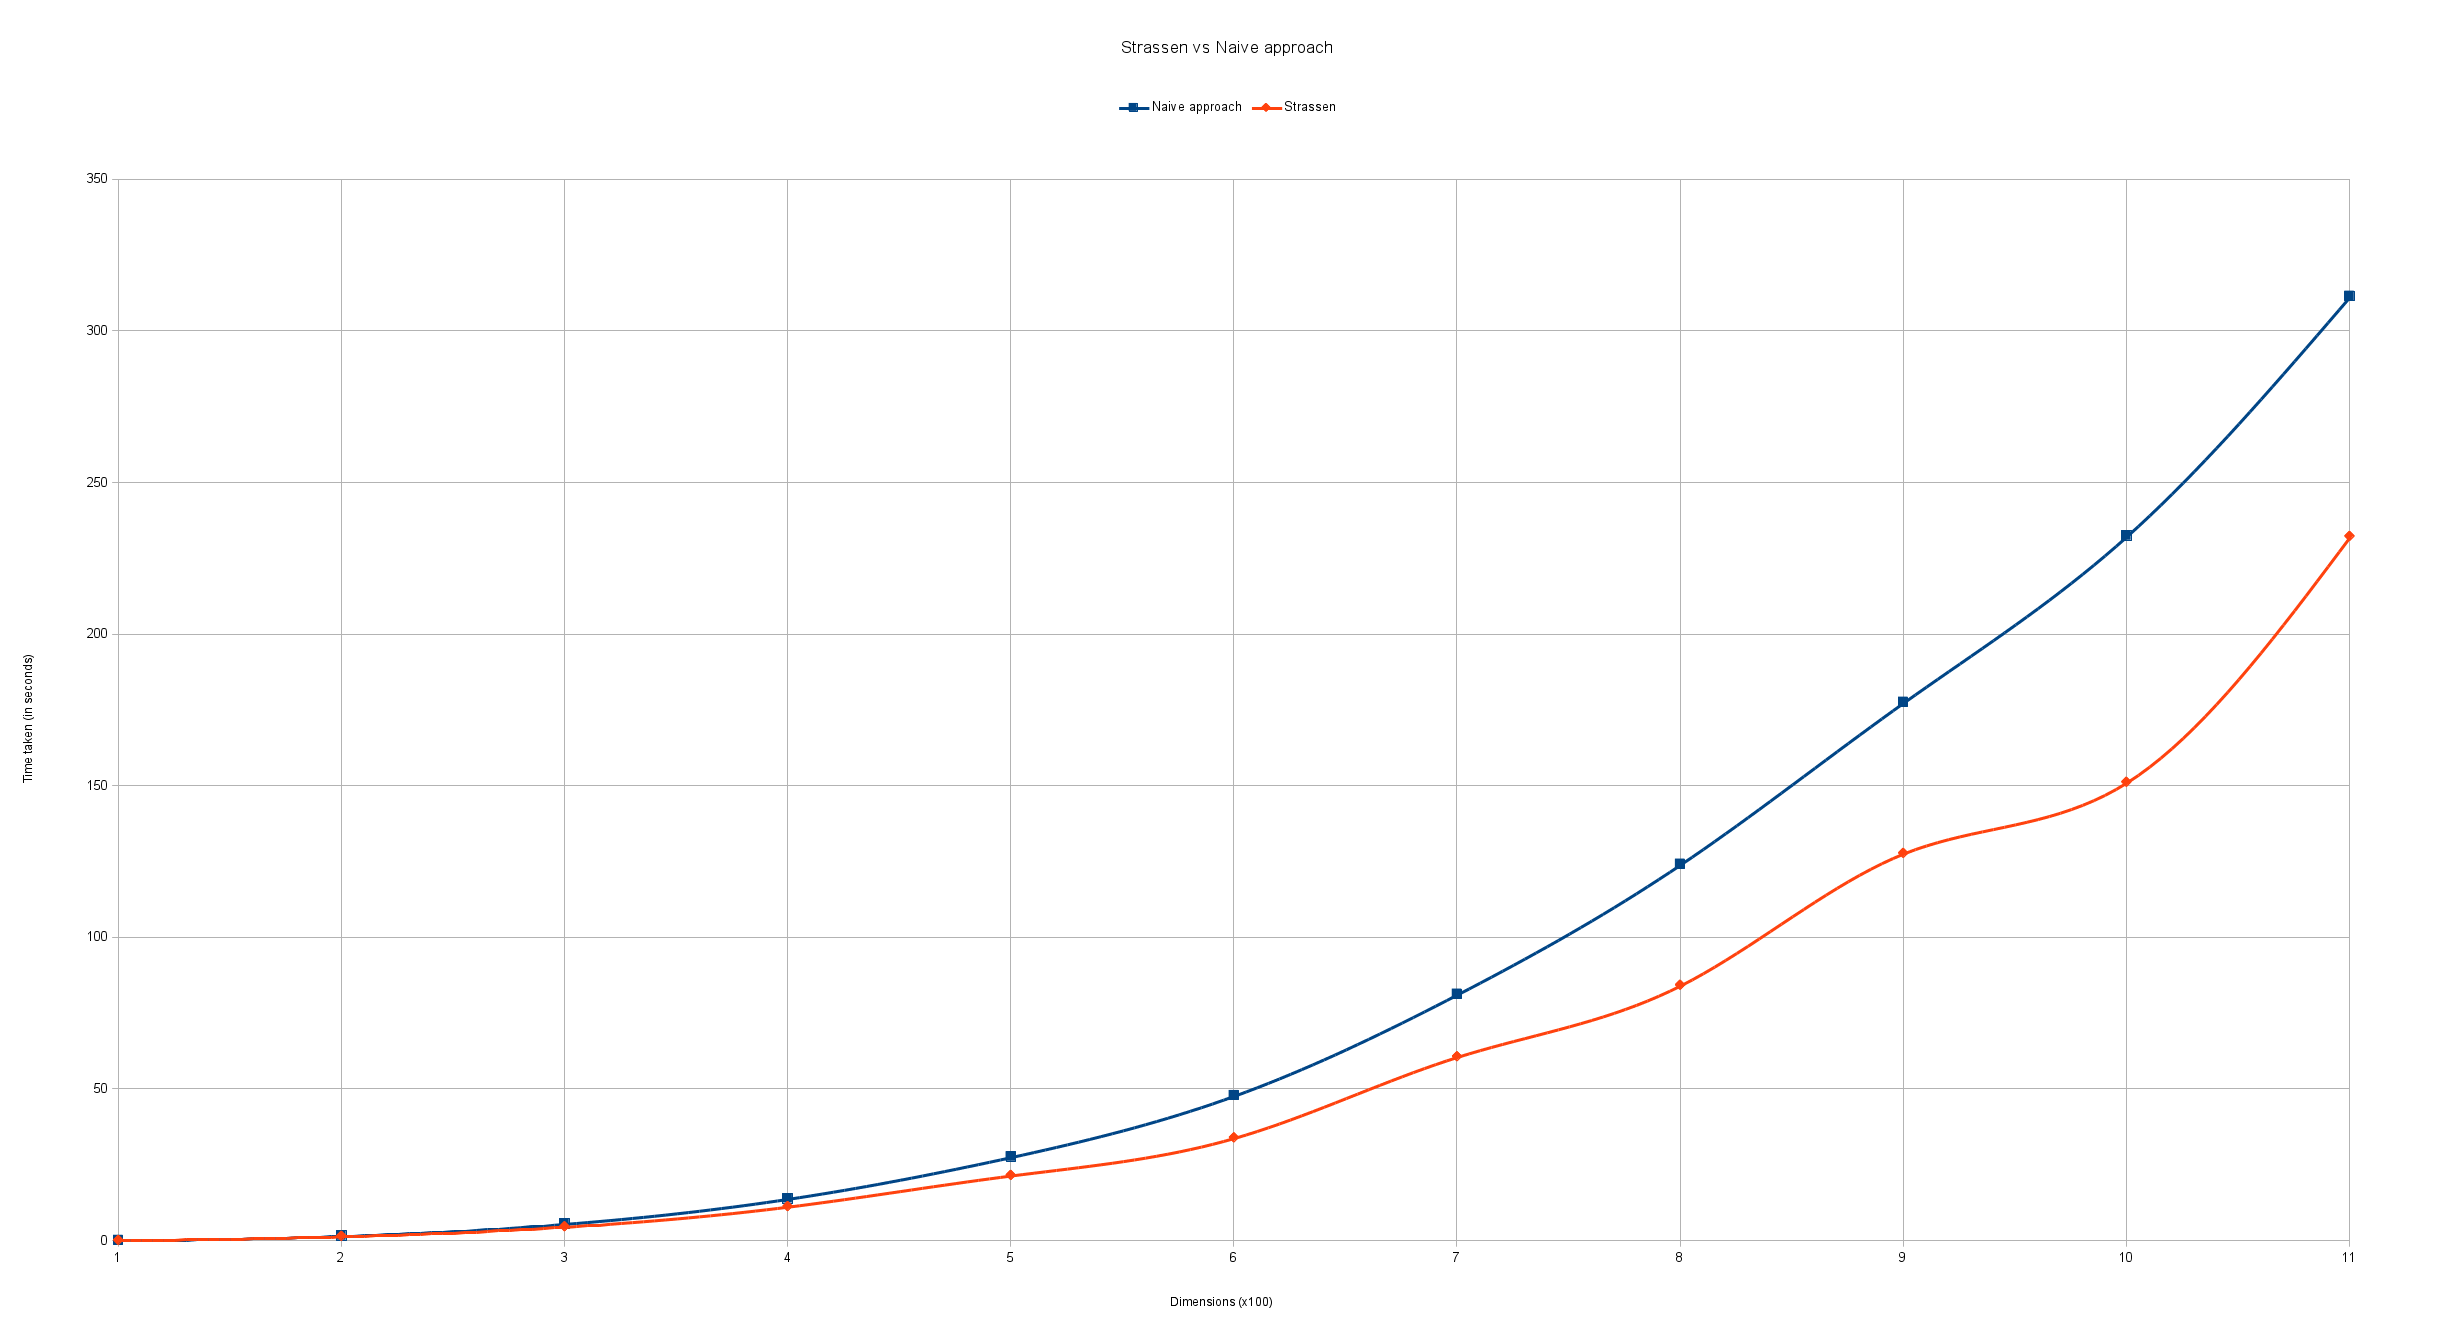
\includegraphics[scale=.75]{char.png} 
\end{flushleft}

\end{document}
